\begin{figure*}[ht]
    \vspace*{-\figskipabove px}
    \vspace*{2px}
	\centering
        
	\begin{subfigure}[t]{0.32\textwidth}
        \centering\vspace{0px}
   		\begin{subfigure}[t]{0.32\textwidth}
   			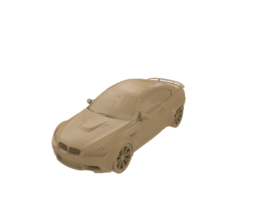
\includegraphics[width=1.75cm,trim={\cropleft cm \croplower cm \cropright cm \cropupper cm},clip]{gdat_shapenet_clean_low_0_ori}
   		\end{subfigure}
   		\begin{subfigure}[t]{0.32\textwidth}
   			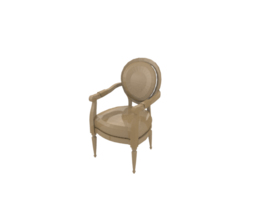
\includegraphics[width=1.75cm,trim={\cropleft cm \croplower cm \cropright cm \cropupper cm},clip]{gdat_modelnet_chair_low_1188_ori}
   		\end{subfigure}
   		\begin{subfigure}[t]{0.32\textwidth}
   			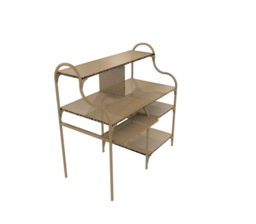
\includegraphics[width=1.75cm,trim={\cropleft cm \croplower cm \cropright cm \cropupper cm},clip]{gdat_modelnet_desk_low_0_ori}
   		\end{subfigure}
        \subcaption{Original}
		\label{fig:data-shapenet-modelnet-a}
	\end{subfigure}
	\begin{subfigure}[t]{0.32\textwidth}
        \centering\vspace{0px}
   		\begin{subfigure}[t]{0.32\textwidth}
   			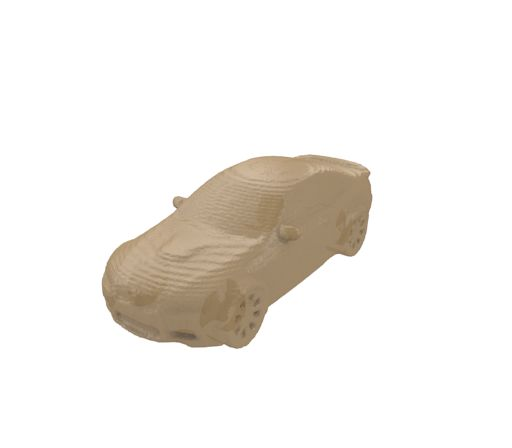
\includegraphics[width=1.75cm,trim={\cropleft cm \croplower cm \cropright cm \cropupper cm},clip]{gdat_shapenet_clean_low_0_wt}
   		\end{subfigure}
   		\begin{subfigure}[t]{0.32\textwidth}
   			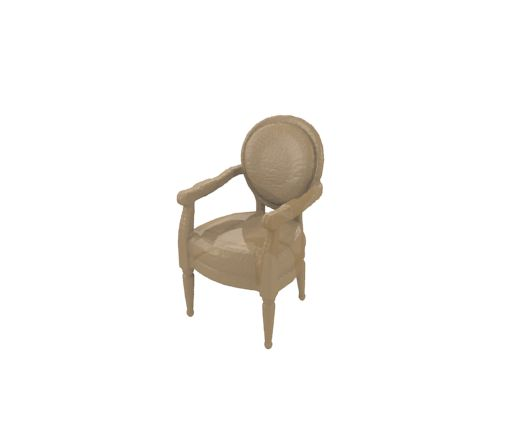
\includegraphics[width=1.75cm,trim={\cropleft cm \croplower cm \cropright cm \cropupper cm},clip]{gdat_modelnet_chair_low_1188_wt}
   		\end{subfigure}
   		\begin{subfigure}[t]{0.32\textwidth}
   			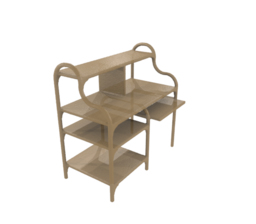
\includegraphics[width=1.75cm,trim={\cropleft cm \croplower cm \cropright cm \cropupper cm},clip]{gdat_modelnet_desk_low_0_wt}
   		\end{subfigure}
        \subcaption{TSDF Fusion, $256^3$}
		\label{fig:data-shapenet-modelnet-b}
	\end{subfigure}
	\begin{subfigure}[t]{0.32\textwidth}
		\centering\vspace{0px}
   		\begin{subfigure}[t]{0.32\textwidth}
   			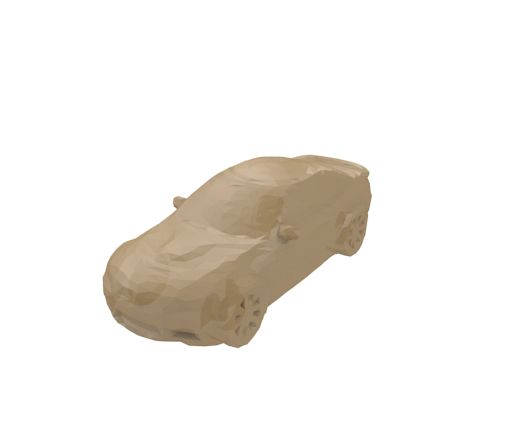
\includegraphics[width=1.75cm,trim={\cropleft cm \croplower cm \cropright cm \cropupper cm},clip]{gdat_shapenet_clean_low_0_simp}
   		\end{subfigure}
   		\begin{subfigure}[t]{0.32\textwidth}
   			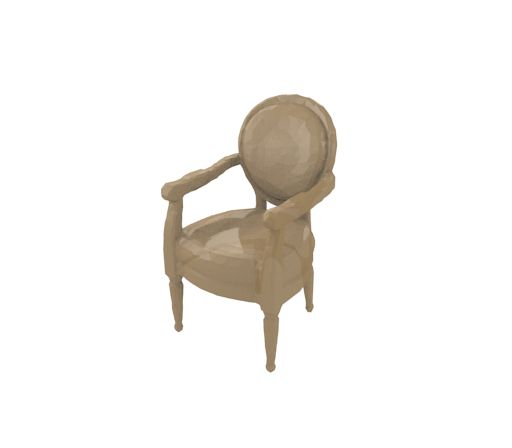
\includegraphics[width=1.75cm,trim={\cropleft cm \croplower cm \cropright cm \cropupper cm},clip]{gdat_modelnet_chair_low_1188_simp}
   		\end{subfigure}
   		\begin{subfigure}[t]{0.32\textwidth}
   			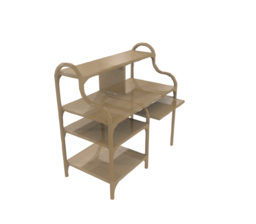
\includegraphics[width=1.75cm,trim={\cropleft cm \croplower cm \cropright cm \cropupper cm},clip]{gdat_modelnet_desk_low_0_simp}
   		\end{subfigure}
        \subcaption{Simplification, $5\text{k}$ Faces}
		\label{fig:data-shapenet-modelnet-c}
	\end{subfigure}
	\\
	\begin{subfigure}[t]{0.32\textwidth}
        \centering\vspace{0px}
   		\begin{subfigure}[t]{0.32\textwidth}
   			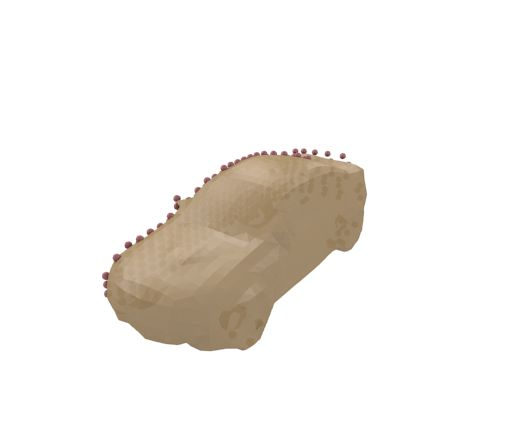
\includegraphics[width=1.75cm,trim={\cropleft cm \croplower cm \cropright cm \cropupper cm},clip]{gdat_shapenet_clean_low_0_rec}
   		\end{subfigure}
   		\begin{subfigure}[t]{0.32\textwidth}
   			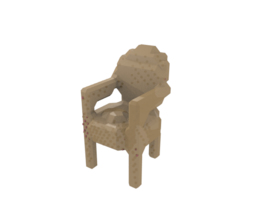
\includegraphics[width=1.75cm,trim={\cropleft cm \croplower cm \cropright cm \cropupper cm},clip]{gdat_modelnet_chair_low_1188_rec}
   		\end{subfigure}
   		\begin{subfigure}[t]{0.32\textwidth}
   			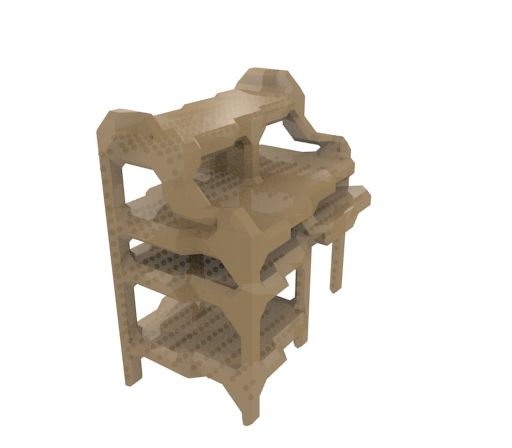
\includegraphics[width=1.75cm,trim={\cropleft cm \croplower cm \cropright cm \cropupper cm},clip]{gdat_modelnet_desk_low_0_rec}
   		\end{subfigure}
        \subcaption{Reconstruction, $24\ntimes54\ntimes24$/$32^3$}
		\label{fig:data-shapenet-modelnet-d}
	\end{subfigure}
	\begin{subfigure}[t]{0.32\textwidth}
        \centering\vspace{0px}
   		\begin{subfigure}[t]{0.32\textwidth}
   			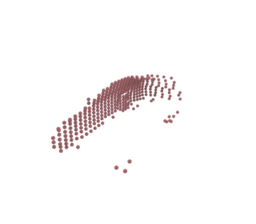
\includegraphics[width=1.75cm,trim={\cropleft cm \croplower cm \cropright cm \cropupper cm},clip]{gdat_shapenet_clean_low_0_points}
   		\end{subfigure}
   		\begin{subfigure}[t]{0.32\textwidth}
   			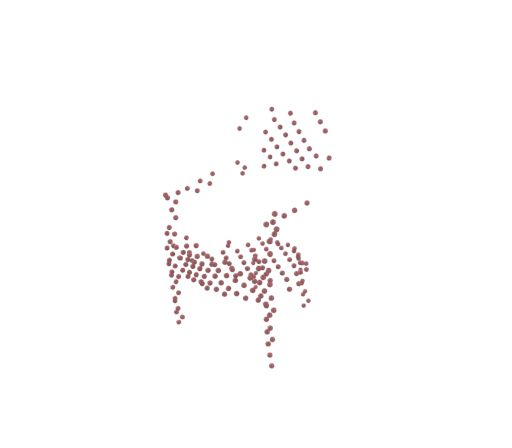
\includegraphics[width=1.75cm,trim={\cropleft cm \croplower cm \cropright cm \cropupper cm},clip]{gdat_modelnet_chair_low_1188_points}
   		\end{subfigure}
   		\begin{subfigure}[t]{0.32\textwidth}
   			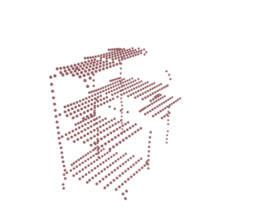
\includegraphics[width=1.75cm,trim={\cropleft cm \croplower cm \cropright cm \cropupper cm},clip]{gdat_modelnet_desk_low_0_points}
   		\end{subfigure}
        \subcaption{Observations}
		\label{fig:data-shapenet-modelnet-e}
	\end{subfigure}
	\begin{subfigure}[t]{0.32\textwidth}
        \centering\vspace{0px}
   		\begin{subfigure}[t]{0.32\textwidth}
   			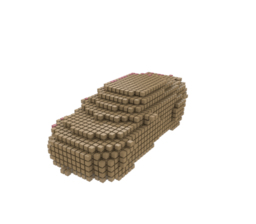
\includegraphics[width=1.75cm,trim={\cropleft cm \croplower cm \cropright cm \cropupper cm},clip]{gdat_shapenet_clean_low_0_bin}
   		\end{subfigure}
   		\begin{subfigure}[t]{0.32\textwidth}
   			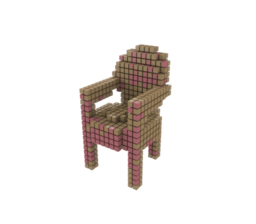
\includegraphics[width=1.75cm,trim={\cropleft cm \croplower cm \cropright cm \cropupper cm},clip]{gdat_modelnet_chair_low_1188_bin}
   		\end{subfigure}
   		\begin{subfigure}[t]{0.32\textwidth}
   			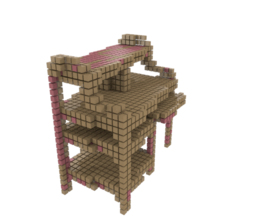
\includegraphics[width=1.75cm,trim={\cropleft cm \croplower cm \cropright cm \cropupper cm},clip]{gdat_modelnet_desk_low_0_bin}
   		\end{subfigure}
        \subcaption{Voxelization, $24\ntimes54\ntimes24$/$32^3$}
		\label{fig:data-shapenet-modelnet-f}
	\end{subfigure}
    \vspace*{-\figskipcaption px}
	\caption{{\bf ShapeNet and ModelNet Data Generation Pipeline.} On ShapeNet and ModelNet we illustrate: {\bf (\subref{fig:data-shapenet-modelnet-a})} samples from the original datasets; {\bf (\subref{fig:data-shapenet-modelnet-b})} fused watertight meshes from TSDF fusion at $256^3$ voxels resolution using \citep{Riegler2017THREEDV}; {\bf (\subref{fig:data-shapenet-modelnet-c})} simplified meshes ($5k$ faces); {\bf (\subref{fig:data-shapenet-modelnet-d})} marching cubes \citep{Lorensen1987SIGGRAPH} reconstructions from the SDFs computed from (\subref{fig:data-shapenet-modelnet-c}) (resolutions $24 \ntimes 54 \ntimes 24$ and $32^3$ voxels; note that steps (\subref{fig:data-shapenet-modelnet-b}) and (\subref{fig:data-shapenet-modelnet-c}) are necessary to derive exact SDFs); {\bf (\subref{fig:data-shapenet-modelnet-e})} observations obtained by projection into a single view; and {\bf (\subref{fig:data-shapenet-modelnet-f})} voxelized observations and shapes. Shapes (meshes and occupancy grids) {in \color{rbeige}beige} and observations in {\color{rred}red}.}
	\label{fig:data-shapenet-modelnet}
    \vspace*{-\figskipbelow px}
\end{figure*}